%!TEX root = ../physical-olympics-2.tex
\chapter{交流电路}


\section{相量表示}

\subsection{拟稳条件与交流元件}

\begin{itemize}
\item 拟稳条件:\,一是忽略传输线上的推迟,\,即传输线的分布电容电感电阻电导都被忽略,\,如果不忽略同一导线两端电流就会不一致且导线将分去电压.\,二是忽略元件内部的推迟.\,不忽略会导致元件非理想.

\item 拟稳条件对应数学表述:
\[\lambda\gg l \quad ,\quad T\gg \frac{l}{c}\]

\item 交流电路瞬时值描述:\,每一瞬时类似直流电路,\,但是电压电流在变化:
\[u=U_0\cos (\omega t+\varphi_u)\]
\[i=I_0\cos (\omega t+\varphi_i)\]

直流电路中的图,\,KVL,\,KCL均成立.\,但是多了电容电感两种元件,\,其特性之后介绍.

\item 有效值:
\[U=U_0/\sqrt{2}\quad ,\quad I=I_0/\sqrt{2}\]

有效值存在意义是为了直接算平均功率:
\[P=I^2R =U^2/R=UI\]

\item 交流电路的相量描述:\,
\[\tilde{U}=Ue^{\uj \varphi_u}\]
\[\tilde{I}=Ie^{\uj \varphi_i}\]


\end{itemize}

\subsection{电阻, 电容, 电感特性}

\begin{itemize}
\item 复阻抗:
\[\tilde{Z}=\frac{\tilde{U}}{\tilde{I}}\]

两种分解方法:
\[\tilde{Z}=|\tilde{Z}|e^{\uj \arg{\tilde{Z}}}=Ze^{\uj \delta}\]

$Z$称为阻抗,\,$\delta$为余损耗角.

\[\tilde{Z}=R+iX\]

$R$称为电阻,\,$X$称为电抗.

\item 复导纳:
\[\tilde{Y}=\frac{\tilde{I}}{\tilde{U}}\]

两种分解方法:
\[\tilde{Y}=|\tilde{Y}|e^{\uj \arg{\tilde{Y}}}=Ye^{\uj \delta}\]

$Y$称为导纳,\,$\delta$为余损耗角.

\[\tilde{Y}=G+iB\]

$G$称为电导,\,$B$称为电纳.

\item 电阻
\[\tilde{Z}=R\]

\item 电感
\[\tilde{Z}=\uj \omega L\]

$Z_L=\omega L$为感抗.\,任何阻抗若电抗为正称为感抗.

\item 电容
\[\tilde{Z}=- \frac{\uj}{\omega C} \quad ,\quad \tilde{Y}=\uj \omega C\]

$Z_C=\omega C$为容抗.\,任何阻抗若电抗为负称为容抗.

\item 元件功率分为视在功率,\,有功功率,\,无功功率.

视在功率:
\[S=UI=I^2Z\]

有功功率:
\[P=UI\cos\delta=I^2R={\rm Re}(\tilde{U}\tilde{I}^*)=\frac{1}{2}(\tilde{U}\tilde{I}^*+\tilde{U}^*\tilde{I})\]

无功功率:
\[P'=UI|\sin\delta|=I^2 |X|\]

三者关系:
\[P'=P\tan|\delta|\quad ,\quad S^2=P^2+P'^2\]

损耗角:
\[\tan\varepsilon=\frac{P}{P'}=\frac{R}{|X|}\quad ,\quad \pm\delta=\frac{\pi}{2}-\varepsilon\]


\end{itemize}

\section{常见电路}

\subsection{谐振电路}

\begin{figure}[H]
\centering
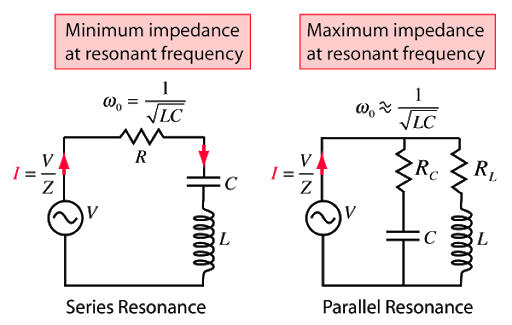
\includegraphics[width=8cm]{image/7-7-1.png}
\caption{串联谐振与并联谐振}
\end{figure}
\begin{itemize}
\item 串联谐振:
\[\tilde{Z}=R+\uj\left(\omega L-\frac{1}{\omega C}\right)\]

谐振条件:\,电流作为响应与电压无相位差:
\[\omega=\frac{1}{\sqrt{LC}}\]

此时恰也有最小阻抗,\,电流最大.

品质因数$Q$:
\[Q=\frac{U_L}{U_R}=\frac{\omega_0 L}{R}=\frac{\omega_0}{\Delta \omega}\]

\item 并联谐振:\,谐振一般定义为相位谐振点,\,即电流作为响应与电压无相位差.\,此时阻抗一般接近最大值,\,故干路电流反而较小.\,支路电路往往远大于干路电流.\,振幅达最小值的振幅谐振点一般不与相位谐振点重合.



\end{itemize}

%\subsection{滤波电路}



%\subsection{电报线方程, 再论拟稳条件}

%\section{变压器}

%\subsection{磁路定律}



%\subsection{理想变压器条件}


%\section{电能传输}

%\subsection{发电机与电动机:\,三相绕组}

%\subsection{变电站与电线损耗}

%\subsection{市电规范}

%\subsection{电源适配器}
